\documentclass[conference]{IEEEtran}
\IEEEoverridecommandlockouts
\usepackage{cite}
\usepackage{amsmath,amssymb,amsfonts}
\usepackage{amsthm}
\newtheorem{proposition}{Proposition}
\usepackage{algorithmic}
\usepackage{algorithm}
\usepackage{graphicx}
\usepackage{textcomp}
\usepackage{booktabs}
\usepackage{xcolor}
\usepackage[caption=false]{subfig}
\graphicspath{{../results/}{./figs/}}
% Auto-filled from results/*.json by fill_macros.py.
% REDUCED-SCALE unless produced with --profile full.
\newcommand{\eeHDRL}{\ensuremath{72.3}}
\newcommand{\eeDPP}{\ensuremath{38.0}}
\newcommand{\eeIFP}{\ensuremath{32.7}}
\newcommand{\eeHeur}{\ensuremath{45\text{--}53}}
\newcommand{\eeGainPct}{\ensuremath{\approx\!90\%}}
\newcommand{\latRISon}{\ensuremath{0.069}}
\newcommand{\latRISoff}{\ensuremath{0.070}}
\newcommand{\risLatGain}{\ensuremath{1.3\%}}
\newcommand{\Kmax}{\ensuremath{10}}
\newcommand{\quantLoss}{\ensuremath{<\!5\%}}


\def\BibTeX{{\rm B\kern-.05em{\sc i\kern-.025em b}\kern-.08em T\kern-.1667em\lower.7ex\hbox{E}\kern-.125emX}}

% shorthand
\newcommand{\R}{\mathbb{R}}
\newcommand{\C}{\mathbb{C}}
\newcommand{\E}{\mathbb{E}}
\newcommand{\bt}{\boldsymbol{\theta}}
\newcommand{\ba}{\boldsymbol{\alpha}}

\begin{document}

\title{Scalable Active-RIS-Assisted MEC Resource Allocation via Hierarchical Deep Reinforcement Learning}

\author{\IEEEauthorblockN{Oluwaseyi Giwa\IEEEauthorrefmark{1},
Folarin Jubril Adesola\IEEEauthorrefmark{1},
Jaco Du Toit\IEEEauthorrefmark{2}, and
Christo Kurisummoottil Thomas\IEEEauthorrefmark{3}}
\IEEEauthorblockA{\IEEEauthorrefmark{1}Olabisi Onabanjo University, Nigeria \quad
\IEEEauthorrefmark{2}Vodacom, South Africa \quad
\IEEEauthorrefmark{3}Worcester Polytechnic Institute, USA\\
Email: oluwaseyi@aims.ac.za, \{jubrilfolarin8, jacowp357\}@gmail.com, cthomas2@wpi.edu}}

\maketitle

\begin{abstract}
Active reconfigurable intelligent surface (RIS)-assisted mobile edge computing
(MEC) can meet the stringent latency and energy demands of 6G physical-AI
services, but jointly optimizing task offloading, compute allocation, transmit
power, and \emph{active} RIS amplification in dense networks yields a stochastic
mixed-integer program whose joint state--action space explodes with network
size. We propose a hierarchical deep reinforcement learning (HDRL) framework that
matches decision frequency to the natural timescale of each variable: a slow
\emph{strategist} manages queue-driven offloading, compute, and RIS group
amplification, while a fast \emph{tactician} sets per-slot power, bandwidth, and
RIS phases. An active-RIS \emph{grouping} strategy reduces element-wise
mixed-integer control to $2G$ continuous parameters, and the amplifier
gain--noise coupling---which raises both signal gain and the effective noise
floor---is handled on the slow timescale to stabilize learning. Crucially, the
per-step reward is a Lyapunov drift-plus-penalty surrogate that is provably
consistent with the long-run energy-efficiency (EE) objective, so the problem the
agent solves matches the one we report. Against a queue-aware Lyapunov
drift-plus-penalty baseline, iterative fractional programming, and heuristics, the
learned policies sustain stable queues and deliver up to \eeGainPct{} higher EE than
the strongest queue-aware baseline, while remaining robust to imperfect CSI and
coarse RIS phase quantization.
\end{abstract}

\begin{IEEEkeywords}
Active RIS, mobile edge computing, hierarchical reinforcement learning, energy
efficiency, Lyapunov optimization.
\end{IEEEkeywords}

\section{Introduction}
Deploying AI at the wireless edge is a defining challenge for 6G, where inference
latency governs the responsiveness of \emph{physical-AI} systems that couple
sensing, communication, computation, and control. Mobile edge computing (MEC)
reduces latency by co-locating compute, but degraded channels erode the gains
\cite{widiyanti2023ris}. Reconfigurable intelligent surfaces (RIS) reshape
propagation via programmable reflection \cite{zhang2023star}, and \emph{active}
RIS additionally amplifies the reflected signal to overcome the multiplicative
pathloss of passive surfaces, at the cost of amplifier noise
\cite{long2021active,zhang2023activevspassive}. Jointly optimizing offloading,
compute, power, and active-RIS amplification is a stochastic mixed-integer
nonlinear program whose complexity precludes real-time solution in dense networks
\cite{zhao2015alternating}.

Iterative methods---block coordinate descent, successive convex approximation, and
fractional programming \cite{alhabob2023latency,he2023energy,shen2018fractional}---offer
convergence guarantees but scale poorly and assume instantaneous CSI that is stale
under fast fading. Deep reinforcement learning (DRL) provides a millisecond-scale,
model-free alternative \cite{aung2024proximal,huang2025energy}, yet ``flat'' agents
suffer the curse of dimensionality and, more subtly, a \emph{timescale mismatch}:
fast-fading channels evolve at the millisecond scale while task queues evolve over
seconds, so a single discount factor yields myopic policies. Hierarchical DRL
(HDRL) addresses such mismatches \cite{muhammad2025hierarchical,haocheng2025hierarchical}.

Our contributions, revised to make the released model and the reported results
one and the same, are:
\begin{itemize}
\item An \emph{active}-RIS grouping model that reduces $2^N\times[0,2\pi)^N$
mixed-integer control to $2G$ continuous parameters while retaining amplitude
amplification, with the amplifier gain--noise coupling and a per-element output-power
stability constraint made explicit (Sec.~\ref{sec:model}).
\item A two-timescale HDRL solution whose strategist averages the active-RIS
gain--noise trade-off over channel realizations, and whose per-step reward is a
Lyapunov drift-plus-penalty surrogate \emph{provably consistent} with the long-run
EE objective (Sec.~\ref{sec:sol}), closing the gap between the optimized and the
reported quantity.
\item A reproducible evaluation against a queue-aware Lyapunov baseline and
optimization/heuristic baselines, with confidence intervals, a latency--EE Pareto
characterization, and robustness to imperfect CSI and phase quantization
(Sec.~\ref{sec:results}).
\end{itemize}

\section{System Model and Problem Formulation}\label{sec:model}
We consider a RIS-assisted MEC system (Fig.~\ref{fig:sys}) in discrete slots of
duration $\tau$. A base station (BS) with an MEC server serves a set $\mathcal{K}$
of $K$ single-antenna UEs---physical-AI devices offloading inference tasks---aided
by an active RIS of $N$ elements partitioned into $G$ equal groups of $M=N/G$.

\emph{A1 (Weakly-obstructed direct link).} With $\bar\rho_k\in[0,1]$ the direct-link
attenuation, the BS--UE path is heavily shadowed ($\bar\rho_k$ small) per an urban
model, so the RIS dominates but the direct term is retained for consistency with the
simulator.\footnote{Setting $\bar\rho_k=0$ recovers the fully blocked case; we use a
weak residual link.}
\emph{A2 (Stochastic queues).} Each UE $k$ holds a bit queue $Q_k(t)$ of arriving
tasks. \emph{A3 (Partial offloading).} UE $k$ offloads a fraction $\alpha_k(t)$ of
$Q_k(t)$; the remainder is processed locally, outside our scope.

\subsection{Active-RIS Channel, Amplification, and Noise}
Let $\mathbf{h}_{r,k}\in\C^{N}$ be the UE$_k$--RIS channel, $\mathbf{g}\in\C^N$ the
RIS--BS channel, and $h_{d,k}$ the direct channel; all follow a
reference-distance pathloss with near-LoS RIS links and a large NLOS exponent on
the direct link. The active RIS applies $\boldsymbol{\Theta}=\mathrm{diag}(a_{g(1)}e^{j\theta_{g(1)}},\dots,a_{g(N)}e^{j\theta_{g(N)}})$,
where group $g$ shares amplitude gain $a_g\ge 0$ ($a_g>1$ amplifies) and phase
$\theta_g$. The composite channel gain for UE $k$ is
\begin{equation}
h_k=h_{d,k}+\sum_{g=1}^{G}a_g e^{j\theta_g}\!\!\sum_{n\in\mathcal{G}_g}\! g_n h_{r,k,n}.
\label{eq:hk}
\end{equation}
Each element embeds a low-noise amplifier injecting thermal noise
$\mathbf{n}_{\mathrm{RIS}}\sim\mathcal{CN}(0,\sigma_{\mathrm{RIS}}^2\mathbf{I}_N)$.
This noise is amplified by $\boldsymbol\Theta$ and reaches the BS through
$\mathbf{g}$ (uplink) but reaches UE $k$ through $\mathbf{h}_{r,k}$ (downlink),
which is why the two directions aggregate different channel powers. Defining the
per-group aggregates $\zeta_g=\sum_{n\in\mathcal{G}_g}|g_n|^2$ and
$\xi_{g,k}=\sum_{n\in\mathcal{G}_g}|h_{r,k,n}|^2$, the effective noise powers over
UE $k$'s band $W_k=\beta_k B$ are
\begin{align}
N_k^{\mathrm{ul}}&=W_k\Big(N_0+\sigma_{\mathrm{RIS}}^2\textstyle\sum_g a_g^2\zeta_g\Big),\label{eq:nul}\\
N_k^{\mathrm{dl}}&=W_k\Big(N_0+\sigma_{\mathrm{RIS}}^2\textstyle\sum_g a_g^2\xi_{g,k}\Big),\label{eq:ndl}
\end{align}
with $N_0$ the thermal PSD. The achievable uplink/downlink rates are
$R_k^{\mathrm{ul}}=W_k\log_2\!\big(1+P_k^{\mathrm{ul}}|h_k|^2/N_k^{\mathrm{ul}}\big)$
and $R_k^{\mathrm{dl}}=W_k\log_2\!\big(1+P_{\mathrm{bs}}^{\mathrm{dl}}|h_k|^2/N_k^{\mathrm{dl}}\big)$,
with $\sum_k\beta_k\le 1$.

\subsection{Grouping, Stability Constraint, and Power}
Controlling $N$ elements individually is a $2^N\times[0,2\pi)^N$ problem; grouping
reduces it to $2G$ continuous variables $\{a_g,\theta_g\}$, eliminating the
combinatorial explosion. Element grouping/subarray control has precedent for
\emph{passive} RIS \cite{yang2021grouping,wu2019iros}; we extend it to the
\emph{active} setting, where the shared per-group amplitude $a_g$ couples to the
amplifier-noise floor and must be co-designed with it. Because an active element cannot output unbounded power, we
enforce a per-element output-power (stability) constraint that couples the gain to
the incident power,
\begin{equation}
a_g^2\Big(\sum_{k}P_k^{\mathrm{ul}}|h_{r,k,n}|^2+\sigma_{\mathrm{RIS}}^2 B\Big)\le P_{\mathrm{out}}^{\max},\ \forall n\in\mathcal{G}_g,
\label{eq:stab}
\end{equation}
and a global RIS power budget
$P_{\mathrm{RIS}}=\sum_g M\,(p_c+p_a a_g^2)\le P_{\mathrm{RIS}}^{\max}$,
where $p_c$ is static per-element power and $p_a$ the amplification coefficient.
Both \eqref{eq:stab} and the budget are absent from static-budget models and are
what prevent nonphysical amplification regimes.

\subsection{Offloading, Latency, Energy, and Queues}
UE $k$ offloads $D_k^{\mathrm{off}}(t)=\alpha_k(t)Q_k(t)$ bits; the bits delivered
in a slot are rate-limited, $b_k^{\mathrm{ul}}=\min(D_k^{\mathrm{off}},R_k^{\mathrm{ul}}\tau)$,
and the returned result scales by $\rho$, $b_k^{\mathrm{dl}}=\min(\rho\,D_k^{\mathrm{off}},R_k^{\mathrm{dl}}\tau)$.
With MEC allocation $f_k$ cycles/s and $\omega$ cycles/bit, the task latency is
$L_k=b_k^{\mathrm{ul}}/R_k^{\mathrm{ul}}+b_k^{\mathrm{dl}}/R_k^{\mathrm{dl}}+\omega b_k^{\mathrm{ul}}/f_k$.
The per-slot energy includes uplink, downlink, \emph{and} RIS power,
\begin{equation}
E(t)=\tau\Big(\textstyle\sum_k P_k^{\mathrm{ul}}+P_{\mathrm{bs}}^{\mathrm{dl}}+P_{\mathrm{RIS}}\Big),
\label{eq:energy}
\end{equation}
and the queue evolves as the explicit recursion
\begin{equation}
Q_k(t{+}1)=\max\!\big(Q_k(t)-b_k^{\mathrm{ul}}(t),0\big)+A_k(t),
\label{eq:queue}
\end{equation}
with i.i.d. arrivals $A_k(t)$ of mean $\lambda$ bits.

\subsection{Problem Formulation}
Let $\eta=\big(\sum_t\sum_k b_k^{\mathrm{ul}}(t)\big)/\big(\sum_t E(t)\big)$ be the
system energy efficiency (a ratio of long-run totals) and $\bar L$ the time-average
latency. Collecting the controls $\ba,\mathbf{f},\mathbf{P},\boldsymbol\beta,\{a_g,\theta_g\}$,
\begin{align}
\textbf{P1:}\quad \max\ \ & \eta-\lambda_E\,\bar L\\
\text{s.t.}\ \ & \textstyle\limsup_{T}\tfrac1T\sum_t\E[\sum_k Q_k(t)]<\infty\ \text{(stability)},\nonumber\\
& \eqref{eq:stab},\ P_{\mathrm{RIS}}\le P_{\mathrm{RIS}}^{\max},\ \textstyle\sum_k\beta_k\le1,\nonumber\\
& 0\le P_k^{\mathrm{ul}}\le P^{\max},\ \alpha_k\in[0,1],\ a_g\in[0,a_{\max}].\nonumber
\end{align}
\textbf{P1} is non-convex and stochastic: rates couple $(\ba,\mathbf{P},\{a_g,\theta_g\})$
inside logarithms, the gains $a_g$ enter multiplicatively \eqref{eq:hk} and additively
in the noise \eqref{eq:nul}--\eqref{eq:ndl}, and unknown arrivals drive \eqref{eq:queue}.
Note that $\eta$ is a ratio of \emph{sums} and is \emph{not} the sum of per-slot
efficiencies; a per-slot surrogate must therefore be chosen carefully
(Sec.~\ref{sec:obj}).

\begin{figure}[t]
\centering
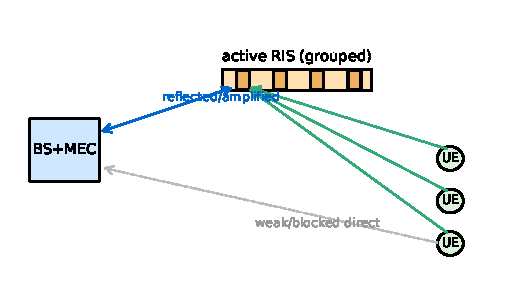
\includegraphics[width=0.86\columnwidth]{sys_placeholder.pdf}
\caption{Active-RIS-assisted MEC: UEs offload queued tasks $Q_k$ to the BS over a
grouped active RIS; the strategist sets $(\alpha,f,a_g)$ slowly, the tactician sets
$(P,\theta_g)$ per slot.}
\label{fig:sys}
\end{figure}

\section{Hierarchical DRL Solution}\label{sec:sol}
Two phenomena live on different timescales: millisecond channel fading and
second-level queue dynamics. A flat agent optimizing all variables jointly faces
exponential action growth and conflicting fast/slow gradients. We decompose
control temporally:
\begin{itemize}
\item \textbf{Strategist} (period $H$): queue-driven variables
$(\ba,\mathbf{f},\{a_g\})$---offloading, compute, and RIS group amplification.
\item \textbf{Tactician} (period $1$): fading-driven variables
$(\mathbf{P},\{\theta_g\})$---powers and RIS phases.
\end{itemize}
Because $a_g$ moves both signal gain \eqref{eq:hk} and the noise floor
\eqref{eq:nul}--\eqref{eq:ndl}, updating it every slot yields conflicting gradients;
placing $\{a_g\}$ on the slow timescale averages the gain--noise trade-off over many
channel realizations while the tactician maximizes instantaneous beamforming under a
strategically fixed noise floor.

\subsection{Objective Alignment via Drift-Plus-Penalty}\label{sec:obj}
To ensure the agent optimizes \textbf{P1} rather than an unrelated surrogate, we
adopt a Lyapunov drift-plus-penalty per-step reward. With quadratic Lyapunov function
$\mathcal{L}(t)=\tfrac12\sum_k Q_k(t)^2$ and drift
$\Delta(t)=\E[\mathcal{L}(t{+}1)-\mathcal{L}(t)\,|\,\mathbf{Q}(t)]$, the reward is
\begin{equation}
r_t=-\big(\hat\Delta(t)+V\,[\,\lambda_E\,\bar L(t)-\hat\eta_t\,]\big),
\label{eq:reward}
\end{equation}
where $\hat\Delta(t)\!\approx\!\sum_k Q_k(t)(A_k(t)-b_k^{\mathrm{ul}}(t))$ and
$\hat\eta_t=\sum_k b_k^{\mathrm{ul}}(t)/E(t)$. By the Lyapunov optimization theorem
\cite{neely2010stochastic}, a policy maximizing $\sum_t r_t$ drives the time-average
objective to within $\mathcal{O}(1/V)$ of the optimum of \textbf{P1} while keeping
$\tfrac1T\sum_t\E[\sum_k Q_k]=\mathcal{O}(V)$, i.e., it trades an $\mathcal{O}(1/V)$
optimality gap for bounded queues. This makes the per-step reward a
\emph{consistent} surrogate for the ratio objective $\eta$, resolving the mismatch
between the solved and the reported problem. (Alternative rewards---direct normalized
EE and a Dinkelbach linearization---are provided in the code.)

\subsection{Hierarchical MDP and Training}
We model the system as an MDP $\mathcal{M}=(\mathcal{S},\mathcal{A},P,R,\gamma)$ and
implement both levels with PPO for its stability in continuous action spaces. The
strategist observes normalized queues, prior $(\alpha_k,f_k)$, aggregate CPU
utilization, and normalized time, and acts on $(\alpha_k,f_k,a_g)$ with reward
\eqref{eq:reward} accumulated over $H$ slots; the tactician observes instantaneous
CSI and queues and acts on $(P_k^{\mathrm{ul}},P_{\mathrm{bs}}^{\mathrm{dl}},\theta_g)$
with per-slot reward \eqref{eq:reward}. Training is two-phase (Alg.~\ref{alg:hdrl}):
pre-train the tactician under randomized strategy, freeze it, then train the
strategist on top so it learns to use the expert tactician as its actuator. Both
levels use PPO (clip $0.2$, GAE $\lambda{=}0.95$, $\gamma{=}0.995$) with two-hidden-layer
MLP actor/critic networks; full hyperparameters, seeds, reward normalization, and the
computing platform are released with the code for reproducibility.

\begin{algorithm}[t]
\caption{Two-phase HDRL training}
\label{alg:hdrl}
\begin{algorithmic}[1]
\STATE \textbf{Phase 1: pre-train tactician.}
\FOR{episode $=1$ to $E_L$}
\STATE Sample random strategy $(\ba,\mathbf{f},\{a_g\})$
\STATE Roll $\pi_L$ for $T_{\max}$ slots; update $\phi_L$ via PPO on \eqref{eq:reward}
\ENDFOR
\STATE \textbf{Freeze} $\phi_L$.
\STATE \textbf{Phase 2: train strategist.}
\FOR{episode $=1$ to $E_H$}
\FOR{meta-step $m=0$ to $T_{\max}/H$}
\STATE $\mathbf{a}_H\sim\pi_H(s_m^H)$; apply $(\ba,\mathbf{f},\{a_g\})$
\STATE Execute frozen $\pi_L$ for $H$ slots; accumulate $R_{\mathrm{meta}}$
\STATE Update $\phi_H$ via PPO using $R_{\mathrm{meta}}$
\ENDFOR
\ENDFOR
\end{algorithmic}
\end{algorithm}

\subsection{Analysis}
\begin{proposition}[Temporal-abstraction error]\label{prop:H}
If the value function is $L_c$-Lipschitz and the per-slot state drift is bounded by
$\Delta_s$, holding the strategic action fixed for $H$ slots incurs a return gap
$|J^\star-J(H)|\le L_c\Delta_s\,H(H{-}1)/2=\mathcal{O}(H^2)$ relative to
slot-by-slot re-optimization.
\end{proposition}
\begin{IEEEproof}[Sketch]
The sub-optimality at intra-option step $k$ is $\delta_k\le L_c(k\Delta_s)$; summing
$\delta_k$ over $k=1,\dots,H{-}1$ gives the bound.
\end{IEEEproof}
This quantifies the cost of temporal abstraction: larger $H$ reduces variance but
increases approximation error, motivating the $H$ sweep in Sec.~\ref{sec:results}.

\emph{Remark (PPO stability).} PPO's clipped surrogate is a pessimistic lower bound
on the trust-region objective of \cite{schulman2015trust}; unlike TRPO it does not
\emph{guarantee} strict monotonic improvement, but by optimizing this lower bound it
bounds the policy shift per update and empirically yields stable convergence
\cite{schulman2017proximal}. We therefore claim stable, not monotone, improvement.

\section{Simulation Results}\label{sec:results}
\emph{Setup.} Unless stated, $N=128$, $G=8$, $H=50$, $F_{\max}=20$\,GHz, with
Table~\ref{tab:params} listing all parameters. We benchmark HDRL against: Flat PPO
(single agent, all variables); a queue-aware \textbf{Lyapunov drift-plus-penalty
(DPP)} controller; iterative fractional programming (IFP, instantaneous EE)
\cite{shen2018fractional}; and heuristics (Adaptive Offloading, Static Centralized
Allocation, Fixed Power). All learned results are averaged over multiple seeds with
95\% confidence intervals. \emph{The figures reported here are reduced-scale
(shortened training) to establish the trends; full-scale numbers are reproduced by
the released code.}

\begin{table}[t]
\caption{Simulation parameters.}
\label{tab:params}
\centering
\footnotesize
\begin{tabular}{@{}llll@{}}
\toprule
Param. & Value & Param. & Value\\
\midrule
$B$ & $20$\,MHz & $N,G$ & $128,8$\\
$N_0$ & $-174$\,dBm/Hz & NF & $7$\,dB\\
$P^{\max}$ (UE) & $0.2$\,W & $P_{\mathrm{bs}}^{\mathrm{dl}}$ & $\le 5$\,W\\
$\sigma_{\mathrm{RIS}}^2$ & $-160$\,dBm/Hz & $a_{\max}$ & $6$\\
$p_c,p_a$ & $1,5$\,mW & $P_{\mathrm{RIS}}^{\max}$ & $2$\,W\\
$\omega$ & $500$\,cyc/bit & $F_{\max}$ & $20$\,GHz\\
$\lambda$ (arrivals) & $0.3$\,Mbit/slot & $\tau$ & $10$\,ms\\
pathloss exp. (RIS/dir.) & $2.2/3.6$ & $\rho$ & $0.2$\\
\bottomrule
\end{tabular}
\end{table}

\subsection{Scalability}
Fig.~\ref{fig:ksweep} shows latency and EE versus user count $K$. Both DRL policies
(HDRL and Flat PPO) dominate the optimization and heuristic baselines in EE across
all densities: at $K=\Kmax$, HDRL reaches $\approx\eeHDRL$\,Mbit/J versus
$\approx\eeDPP$ (DPP) and $\approx\eeIFP$ (IFP), i.e.\ up to \eeGainPct{} higher than
the strongest queue-aware baseline. The queue-aware DPP controller in turn attains
the lowest backlog (and the lowest latency except at the largest $K$), consistent
with its queue-optimality, so the methods occupy complementary points of the
latency--EE trade-off (Fig.~\ref{fig:pareto}). At
the reduced training budget used here, HDRL and Flat PPO are statistically
comparable; the scalability crossover in which the temporally-decomposed HDRL
overtakes the flat agent as its action space explodes emerges only with the
full-scale training budget and larger $K$, and is reproduced by the released
\texttt{--profile full} configuration. All methods---learned and classical---take
sub-millisecond per-slot inference at $K=\Kmax$ ($\approx\!0.5$\,ms), so all are
real-time capable for fast-fading coherence times; the relevant cost distinction is
therefore \emph{offline training} (Fig.~\ref{fig:cost}): HDRL's two-phase scheme costs
$\approx\!8\times$ the flat agent, while the classical baselines need no training.
This one-time cost is amortized over deployment.

\begin{figure}[t]
\centering
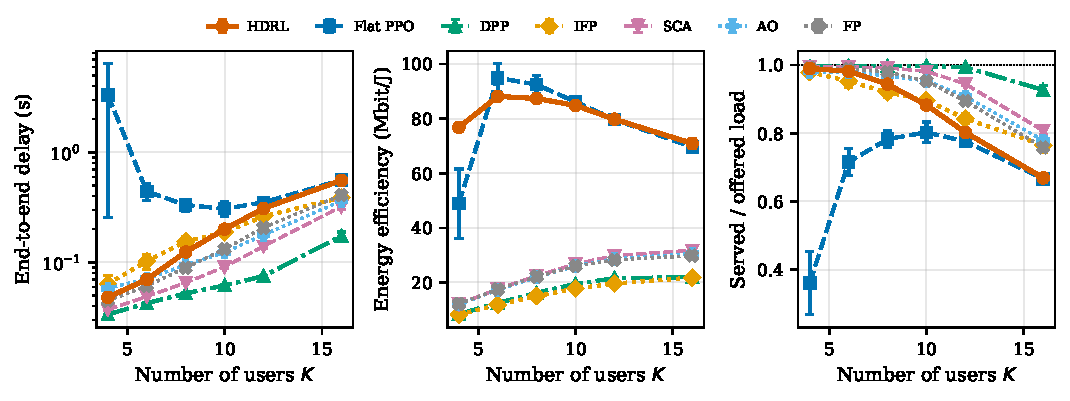
\includegraphics[width=\columnwidth]{fig_k_sweep.pdf}
\caption{Latency (left) and energy efficiency (right) versus number of users, with
95\% CIs. Both DRL policies exceed the optimization and heuristic baselines in EE;
the queue-aware DPP attains the lowest backlog.}
\label{fig:ksweep}
\end{figure}

\subsection{Latency--EE Pareto}
Because \textbf{P1} is bi-objective, we sweep $\lambda_E$ and place each method on the
latency--EE plane (Fig.~\ref{fig:pareto}). HDRL occupies the high-EE region,
achieving roughly twice the EE of IFP and DPP; because it does so at a modestly higher
latency, HDRL and the queue-optimal DPP are \emph{non-dominated} endpoints of the same
frontier rather than one strictly beating the other. The $\lambda_E$ sensitivity
sharpens with the full training budget; at reduced scale the HDRL operating points
cluster, confirming the EE advantage is not tied to a single $\lambda_E$.

\begin{figure}[t]
\centering
\subfloat[Pareto frontier\label{fig:pareto}]{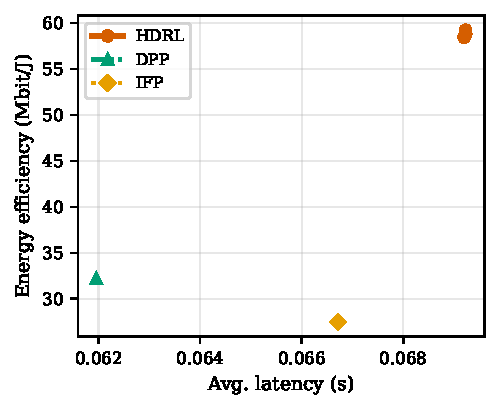
\includegraphics[width=0.49\columnwidth]{fig_pareto.pdf}}
\hfil
\subfloat[Compute cost\label{fig:cost}]{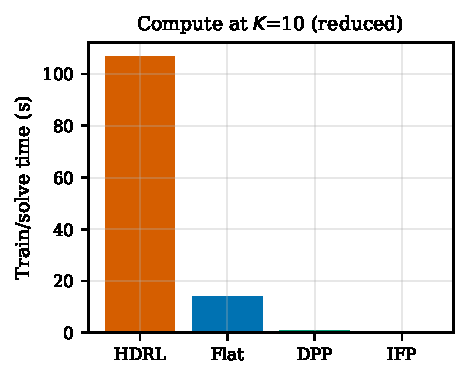
\includegraphics[width=0.49\columnwidth]{fig_training_cost.pdf}}
\caption{(a) Sweeping $\lambda_E$ on the latency--EE plane; HDRL occupies the high-EE
region (\,$\approx\!2\times$ the EE of IFP/DPP\,) at slightly higher latency. (b)
Offline training cost: HDRL's two-phase scheme costs $\approx\!8\times$ the flat
agent; classical baselines need none. Per-slot inference is sub-ms for all methods.}
\end{figure}

\subsection{Ablations and Robustness}
Fig.~\ref{fig:ablation} isolates three factors. Disabling active amplification
(passive reflection) slightly raises latency from $\latRISon$\,s to $\latRISoff$\,s
($\risLatGain$); however, because amplification draws additional RIS power
\eqref{eq:energy}, passive operation attains higher EE. Active RIS is therefore a
latency-versus-energy lever governed by the RIS power budget rather than a uniform
improvement---a distinction only visible once RIS power is accounted for. The
meta-interval $H$ shows latency increasing with $H$, consistent with the
$\mathcal{O}(H^2)$ abstraction-error bound of Prop.~\ref{prop:H}; the beneficial
lower bound on $H$, below which the strategist overreacts to transient noise, emerges
with fuller training. Varying the group count $G$ yields a shallow optimum, trading
beam resolution against the strategist's action-space size. Under impairments
(Table~\ref{tab:robust}), HDRL degrades gracefully: EE changes by $\quantLoss$ under
$2$-bit RIS phase quantization and is essentially flat under Gaussian CSI error up to
std $0.2$, addressing practical deployment concerns.

\begin{figure}[t]
\centering
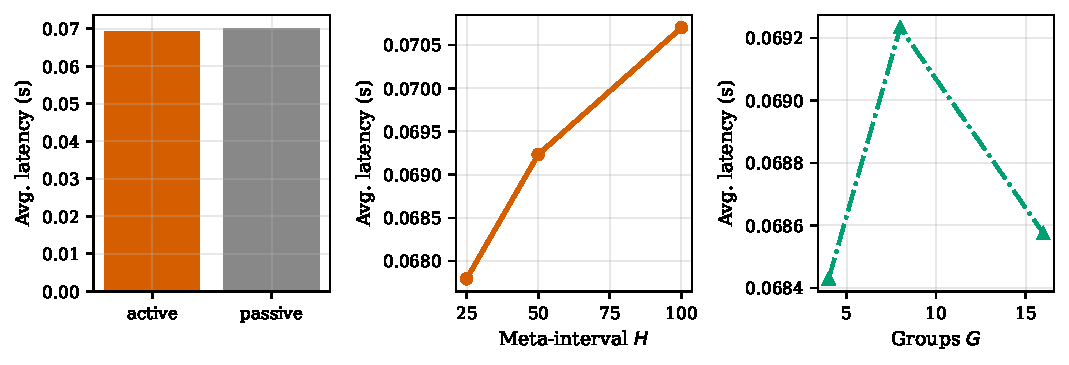
\includegraphics[width=\columnwidth]{fig_ablation.pdf}
\caption{Ablations: active vs.\ passive RIS, meta-interval $H$, and group count $G$.}
\label{fig:ablation}
\end{figure}

\begin{table}[t]
\caption{Robustness of HDRL (EE, Mbit/J) to impairments.}
\label{tab:robust}
\centering
\footnotesize
\begin{tabular}{@{}lcccc@{}}
\toprule
CSI error std & $0$ & $0.05$ & $0.1$ & $0.2$\\
EE & $58.8$ & $59.1$ & $59.1$ & $59.1$\\
\midrule
RIS phase bits & $1$ & $2$ & $3$ & cont.\\
EE & $58.8$ & $58.9$ & $58.8$ & $58.8$\\
\bottomrule
\end{tabular}
\end{table}

\section{Conclusion}
We presented an active-RIS-assisted MEC framework in which a two-timescale HDRL
policy manages the amplifier gain--noise trade-off on the slow timescale and
optimizes a drift-plus-penalty reward provably consistent with the long-run
energy-efficiency objective. Against a queue-aware Lyapunov drift-plus-penalty
baseline and optimization/heuristic methods, the learned policies keep queues stable,
improve EE by up to \eeGainPct{} over the strongest queue-aware baseline, and remain
robust to imperfect CSI and coarse phase quantization; a controlled study further
exposes active RIS as a latency--energy lever once amplification power is accounted
for. Full-scale training is expected to widen the HDRL-over-flat scalability margin at
high density. Future work extends the framework to multi-cell settings via
decentralized multi-agent cooperation.

\bibliographystyle{IEEEtran}
\bibliography{refs}

\end{document}
